% !TeX spellcheck = en_US
\documentclass[]{article}


%opening
\title{Current Topics in Multimedia Communication: Server, Cluster, and Cloud Computing--Project 1}

\author{Giovanni Liva}

\usepackage[T1]{fontenc}
\usepackage[english]{babel}
%\usepackage[utf8]{inputenc}
\usepackage[latin1]{inputenc}
\usepackage{graphicx}
\usepackage{amsmath}
\usepackage{mathtools}
\usepackage{amsfonts}
\usepackage[final]{pdfpages}

\usepackage{hyperref}
\hypersetup{
	colorlinks   = true,    % Colours links instead of ugly boxes
	urlcolor     = blue,    % Colour for external hyperlinks
	linkcolor    = blue,    % Colour of internal links
	citecolor    = red      % Colour of citations
}
\newcommand{\norm}[1]{\left\lVert#1\right\rVert}

\usepackage{wrapfig}
\usepackage{lscape}
\usepackage{rotating}
\usepackage{epstopdf}
\usepackage{float}

\begin{document}

\maketitle


\section*{Introduction}
I create code in C and C++ because i discover after create YSMF that pthread and C++ classes don't works pretty well together

My specs are:
Procio: 2,5 GHz Intel Core i7-4870HQ
num Cores: 8
num Threads: 8
RAM: 16GB

Code in C/C++
How to compile



\section*{Implementation}

C++ class for YSMF
pthread to implement threads
three different strategies
motivation why three 


\section*{Evaluation}

Run \texttt{./evaluation.sh} to generate .csv files.
Then process them with R to generate the following graphs.


\paragraph{all\_single}
blabla
\begin{figure}[H]
	\centering
	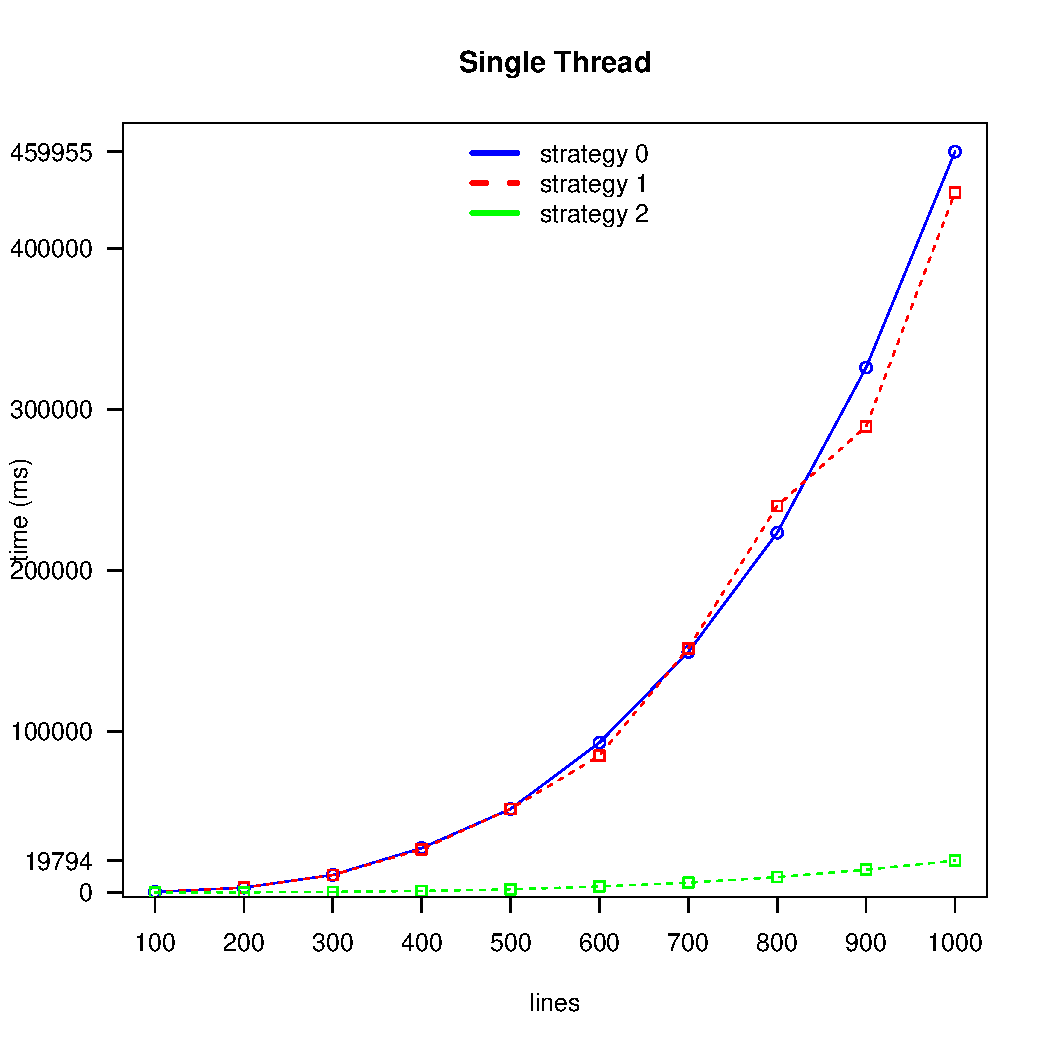
\includegraphics[width=1\textwidth]{img/all_single.pdf}
	\caption
	{RAM Used to compute a matrix $100000\times1000000$}
	\label{fig:all_single}
\end{figure}


\paragraph{all\_multiple}
bla bla bla
\begin{figure}[H]
	\centering
	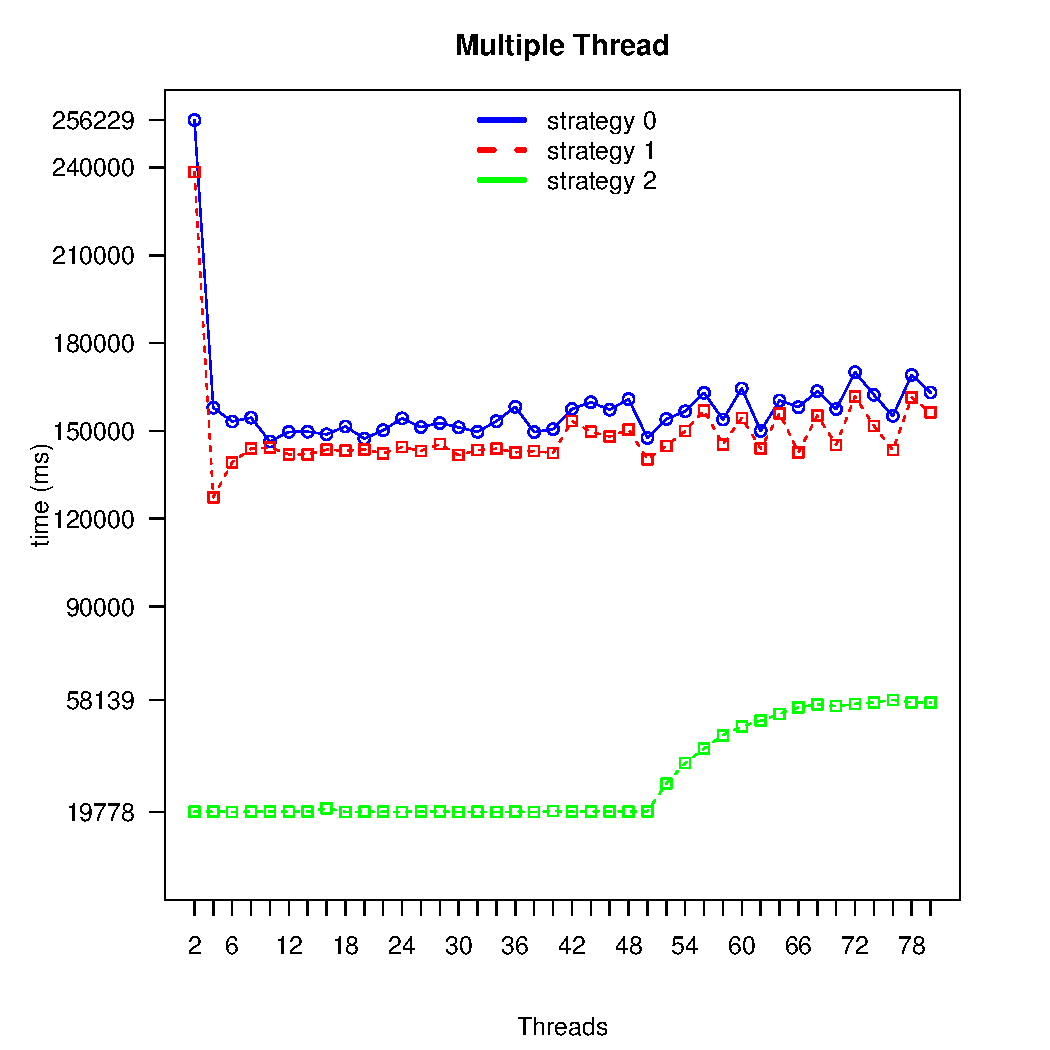
\includegraphics[width=1\textwidth]{img/all_multiple.pdf}
	\caption
	{RAM Used to compute a matrix $100000\times1000000$}
	\label{fig:all_multiple}
\end{figure}



\paragraph{diff\_time\_multiple}

\paragraph{init\_phase}

\paragraph{speedup}


\paragraph{Blow the Memory UP}
$100000\times1000000$
\begin{figure}[h!]
	\centering
	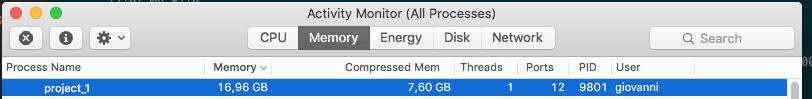
\includegraphics[width=1.15\textwidth]{img/memory_used.png}
	\caption
	{RAM Used to compute a matrix $100000\times1000000$}
	\label{fig:memory_blowed_up}
\end{figure}


\end{document}
